\section{Redes de Sensores Sem Fio}

A capacidade de computação e evolução do hardware se torna exponencialmente barata e de menor tamanho a cada ano. Engenheiros e pesquisadores têm desenvolvido miniaturizações de rádios e estruturas de sensores minúsculas. Estas estruturas são capazes de sensoriar e medir campos e forças do mundo real. Esta motivação abre espaço para que se construam aplicações de medição nos mais diversos cenários. Aliando-se este grande desenvolvimento na área de microeletrônica juntamente com a atual estrutura da internet tem-se um horizonte ainda mais amplo e desafiador \cite{Culler2004}. 

Neste contexto, frente esta nova gama de problemas e aplicações, tem-se as Redes de Sensores Sem Fio.

\wsn  são um conjunto de nós individuais capazes de interagir com o ambiente em que estão inseridos, sensoriando ou controlando parâmetros físicos.
Geralmente, um nó da rede não apresenta capacidades suficientes para cumprir sua tarefa. Portanto, os diversos nós devem desenvolver um comportamento colaborativo para cumprir estas tarefas. Para que se desenvolva este comportamento colaborativo, um meio de comunicação entre estes nós torna-se necessário. São utilizados enlaces sem fio para estabelecer a comunicação entre os nós da rede \cite{Holger2005}.


Segundo \cite{Loureiro}, uma \rssf pode ser vista como um tipo especial de rede móvel ad hoc (MANET - Mobile Ad Hoc Network). De um ponto de vista organizacional, ambas podem ser consideradas idênticas, visto o fato de possuirem elementos computacionais que se comunicam sem fios. Porém, ambas se distinguem em relação às finalidades. As tradicionais redes MANETs podem e devem executar tarefas computacionais distintas, enquanto as \rssfs devem trabalhar colaborativamente, a fim de executarem uma só tarefa global a partir de seus comportamentos locais.

Atualmente, segundo \cite{Holger2005}, as \rssfs são um desafio para a pesquisa e a engenharia. Sua grande flexibilidade e suporte a várias aplicações do mundo real são motivações para o desenvolvimento desta área de pesquisa.
% Não existe um único conjunto de definições que defina exatamente as \rssfs , nem mesmo uma única soluçao técnica que englobe todo o espaço de aplicações.


\rssfs se adaptam a uma grande variedade de problemas do mundo real. Nós sensores podem ser utilizados para medições de temperatura, pressão, umidade, bem como aplicações de monitoramento, vigilância, detecção de desastres, trajetória de alvos e vigilância. Uma \rssf também pode ser distribuída em fábricas para se monitorar vazamento de materiais nocivos ou tóxicos \cite{Aboelaze2005}.


As bases para o desenvolvmento das \rssfs advêm de três principais áreas: sensoriamento, comunicação e computação (hardware, software a algoritmos). Logo, os avanços de cada uma destas áreas (em conjunto ou separadas) têm direcionado a pesquisa em \rssf\cite{Chong2003}. 

\subsection{Desafios das \rssfs}

Atualmente, as RSSFs apresentam alguns desafios, principalmente no tocante à plena utilização de seus recursos. Pelo fato de cada nó apresentar um conjunto limitado de hardware e funcionalidades, a plena utilização dos recursos da rede torna-se então o principal desafio das RSSFs.
\cite{Dressler2007} divide os desafios das RSSFS em:

\begin{description}
\item [Confiabilidade da comunicação sem fio:] Em muitos casos, especialmente com um número crescente de nós no mesmo raio de comunicação, a comunicação sem fio  tende a não ser confiável. A principal causa deste fenômeno é a grande quantidade de colisões entre os pacotes trocados entre os nós. A probabilidade de colisão é proporcional à densidade da rede, o tamanho e tráfego gerado. Confiabilidade é a capacidade de prover garantia de entrega aos pacotes.
			
\item [Mobilidade espaço-temporal:] Mobilidade espacial refere-se à movimentação geográfica dos nós da rede, i.e. mudanças da localização dos nós ao decorrer do tempo.
			
\item [Limitação de recursos:] Problemas como limitação de tempo vida de baterias, \emph{cpus} de poder de processamento de poucos MHz e memórias de alguns KB.
			
\item [Requisitos de tempo real:] Recai sobre a necessidade das aplicações em alguns casos necessitarem de informações em tempo real. Neste caso, torna-se fundamental que a rede de sensores seja capaz de prover informações confiáveis em tempo real.	
\end{description}

Um desafio adicional muito importante é a coordenação em um sistema massivamente distribuído apresentado pelas RSSFs.

\subsection{Tipos de Aplicações}
O desenvolvimento das \rssfs oferece suporte para uma grande variedade de aplicações, principalmente em casos de detecção de parâmetros em ambientes. Aplicações militares, detecção de incêndios, monitoramento de fábricas, recuperação de desastres, agricultura de precisão, etc; são exemplos de aplicações de \rssfs.

\cite{Holger2005} definem quatro principais padrões de operação em redes de sensores. Estes padrões de operações definem os principais tipos de aplicação.

\begin{description}

\item[Detecção de Eventos:] São casos onde os nós sensores devem reportar a detecção de ocorrência de um dado evento de interesse. O caso mais simples de detecção de evento é quando um único nó detecta um evento (algum limite pré-definido é ultrapassado) e deve reportar aos outros nós. Casos mais complexos são os que requerem consenso de vários nós para se determinar a ocorrência de um determinado evento.

\item[Medidas Periódicas: ] São as situações em que os nós têm tarefas somente de medições, reportando periodicamente as informações coletadas. Em alguns casos, estes relatórios podem ser enviados em casos de detecção de eventos. Porém, os critérios sobre os momentos de relatório devem ficar a critério das aplicações.

\item[Aproximação de Funções e Detecção de Bordas:] Uma \rssf pode utilizar amostras de diferentes regiões para estimar parâmetros gerais do ambiente. Um exemplo é o modo como os valores físicos de leitura de temperatura pode variar de uma região para outra. Neste caso, ignorando outros fatores condicionantes, pode-se supor que a medida da temperatura pode ser dada em função da localização. Em consequencia disto, podem ser utilizadas amostragens de temperatura de diferentes regiões para se aproximar esta função desconhecida.

\item[Rastreamento:] A causa de um evento pode ser móvel, como casos de entrada de intrusos em cenários de vigilância. A \rssf pode ser configurada para relatar as atualizações da posição corrente do intruso. Existe também a possibilidade de se estimar a velocidade e direção dos intrusos. 

\end{description}

Uma tendência que tem ganhado força em aplicações de \rssf é a utilização de uma rede com sensores heterogêneos, dentre estes casos, destaca-se o uso de veículos aéreos não tripulados atuando como sensores móveis da rede \cite{Freitas2009}. 


\subsection{Características}
Redes de sensores podem apresentar diferentes características e requisitos. Cada rede apresentará características variadas, pois cada aplicação pode demandar diferentes requisitos.
Este fato obriga a rede de sensores a se preocuparem com fatores específicos.

\cite{Loureiro} discutem algumas características mais relevantes:

\begin{description}
	\item[Endereçamento dos nós sensores:] trata-se de endereçar unicamente um sensor dentro da rede. Existem casos em que se torna necessário saber a localização ou fonte dos dados, como quando são utilizados sensores espalhados em uma fábrica ou no corpo humano. Nesses casos é interessante saber a fonte dos dados. Contudo, em casos onde existe uma infinidade de sensores medindo valores no ambiente pode não ser necessário identificar cada nó individualmente.

	\item[Agregação dos dados:] indica a possibilidade da rede agregar os dados coletados pelo sensor. Ou seja, se os dados serão condesados em um único ponto, ou se serão espalhados e enviados por todos os nós. Se esta funcionalidade (agregação) estiver presente, cria-se a possibilidade de economia de tráfego de mensagens até uma estação base.

	\item[Mobilidade dos Sensores: ] preocupa-se com a mobilidade ou não dos sensores em relação aos sistemas em que se encontram inseridos. Diferentes abordagens devem ser utilizadas em cada caso. 

	\item[Quantidade de Sensores:] aplicações de \rssf podem conter de poucos, à dezenas e à milhares de nós sensores. Uma das maiores preocupações, neste caso, é a escalabilidade do sistema. Combinada com a mobilidade, esta questão pode ser uma das características mais críticas no desenvolvimento de uma aplicação de RSSF.

	\item[Limitação de Energia Disponível: ] em vários casos, as \rssfs são distribuídas em áreas remotas ou de difícil acesso. Nestas ocasiões, a autonomia (tempo de vida) de um sensor restringe-se a somente o tempo de bateria disponível, pois nem sempre se tem a garantia de manutenção na rede. Diversas abordagens e modelos têm sido estudados para se tratar problemas relacionados à autonomia de energia.

	\item[Auto-Organização na rede: ] os nós da rede devem se organizar, de modo com que os fatores externos sejam minimizados, ou seja, a rede deve estar preparada para se recuperar de possíveis falhas e imprevistos. Caso um nó seja removido (por qualquer fator), a rede deve ser capaz de se reconfigurar e prosseguir com suas tarefas.

	\item[Tarefas Colaborativas: ] geralmente, um nó único da rede não possui capacidade para executar tarefas complexas por si próprio. Neste caso, torna-se necessário um comportamento colaborativo na rede, ou seja, vários nós devem colaborar para que se cumpram as tarefas e, consequentemente, sejam alcançados os objetivos da rede em questão.

	\item[Capacidade de responder a consultas: ] uma \rssf deve ser capaz de responder às requisições (\emph{requests}) e às perguntas (\emph{querys}) que lhe são direcionadas. Uma \emph{query} pode ser direcionada a somente um nó, a um grupo de nós ou à toda rede.

\end{description}

\rssfs também podem ser classificadas quanto a sua configuração (tabela \ref{tbl:configuração}), em relação ao tipo de sensoriamento (tabela \ref{tbl:sensoriamento}) e também quanto ao processamento (tabela \ref{tbl:processamento}) \cite{Ruiz2004}.

\pagebreak

\begin{table}[h!]
\centering
\small
	\begin{tabular}{ | l | l | p{8.0cm} | }
		\hline
		\multicolumn{3}{|c|}{\textbf{Configuração}} \\
		\hline

		\multirow{2}{*}{\textbf{Composição}}
				 & Homogênea & É uma rede composta por nós sensores com o mesmo hardware. Isto não implica que o software deve ser o mesmo. \\ 
				\cline{2-3}
			       	& Heterogênea &  A rede é composta por uma variedade de nós com hardware diferente.  \\
		\hline

		\multirow{2}{*}{\textbf{Organização}}
			& Hierárquica & Os nós são organizados em \emph{clusters} de forma hierárquica. Existirão nós líderes a serem eleitos pelos nós comuns.\\
			\cline{2-3}
			& Plana & Todos os nós encontram-se no mesmo nível de hierarquia. \\
		\hline

		\multirow{2}{*}{\textbf{Mobilidade}}
			& Estacionária & Os nós sensores permanecerão todo o tempo no mesmo local onde foram colocados. \\
			\cline{2-3}
			& Móvel & Existe a possibilidade dos nós sensores se deslocarem durante a operação da rede.\\
		\hline

		\multirow{3}{*}{\textbf{Densidade}}
			& Balanceada & Pode ser considerada como uma rede com a concentração e distribuição considerada ideal para a aplicação em questão.\\
			\cline{2-3}
			& Densa & É uma rede que aprensenta uma alta concentração de nós em uma determinada área. \\
			\cline{2-3}
			& Esparsa & Os nós são distribuídos com uma baixa concentração dentro de uma área de interesse. \\
		\hline

		\multirow{2}{*}{\textbf{Distribuição}}
			& Irregular & A distribuição dos sensores não se apresenta uniformemente na área em questão. \\
			\cline{2-3}
			& Regular & É o caso onde os nós sensores estão distribuídos uniformemente pela área de interesse.\\
		\hline
	\end{tabular}

	\caption{Classificação de \rssfs em relação à configuração.}
	\label{tbl:configuração}
\end{table}


\begin{table}[h!]
\centering
\small
	\begin{tabular}{ | l | l | p{8.5cm} | }
		\hline
		\multicolumn{3}{|c|}{\textbf{Sensoriamento}} \\
		\hline

		\multirow{4}{*}{\textbf{Coleta}}
				 & Periódica & A coleta de dados é realizada de forma periódica. Ou seja, de tempos em tempos o nó realiza medições. \\ 
				\cline{2-3}
			       	& Contínua &  Os nós sensores coletam dados continuamente.  \\
				\cline{2-3}
				 & Reativa & Dados são coletados na ocorrência de um evento de interesse, ou no momento em que uma consulta é solicitada por um agente externo. \\ 
				\cline{2-3}
			       	& Tempo Real & Os nós sensores coletam a maior quantidade possivel no menor intervalo de tempo.  \\
		\hline
	\end{tabular}

	\caption{Classificação de \rssfs quanto ao modo de Sensoriamento.}
	\label{tbl:sensoriamento}
\end{table}


\begin{table}[h!]
\centering
\small
	\begin{tabular}{ | l | l | p{7.2cm} | }
		\hline
		\multicolumn{3}{|c|}{\textbf{Processamento}} \\
		\hline

		\multirow{3}{*}{\textbf{Cooperação}}
				 & Infra-Estrutura & São executados processamentos referentes à infra-estrutura da rede, como algoritmos de acesso ao meio, roteamento, eleição de líderes, etc. \\ 
				\cline{2-3}
			       	& Localizada &  Os nós executam funções além das básicas de infra-estrutura como, por exemplo, a tradução de dados capturados pelo sensor.  \\
				\cline{2-3}
				& Correlação & Os nós estão envolvidos em procedimentos de correlação de dados como fusão, supressão seletiva, contagem, compressão, multi-resolução e agregação. \\
		\hline
	\end{tabular}

	\caption{Classificação de \rssfs quanto ao modo de Processamento.}
	\label{tbl:processamento}
\end{table}

\subsection{Nós Sensores}

O hardware de um nó sensor da rede é composto por um microprocessador, uma unidade de armazenamento, sensores, conversores analógico-digital, um transceiver de dados, controladores que unem estas partes, e uma fonte de energia \cite{Culler2004}.

Segundo \cite{Holger2005}, os requisitos das aplicações representam fatores decisivos no que diz respeito a tamanho, custos, e consumo de energia dos nós. Características tais como comunicação e poder de processamento devem ser prover um nível mínimo de qualidade que atenda aos requisitos destas aplicações. Encontrar o equilíbrio entre funcionalidades e custos é uma tarefa crucial na escolha do modelo de nó correto.

\cite{Holger2005} definem a estrutura básica de um nó sensor sem fio como:
\begin{description}
\item[Controlador:] um controlador para processar os dados, capaz de executar códigos arbitrários.
\item[Memória:] unidade de memória para armazenar programas e alguns dados intermediários.
\item[Sensores e Autuadores:] a verdadeira interface com o mundo real, dispositivos que podem observar ou controlar parâmetros físicos do ambiente.
\item[Fonte de Energia:] componente responsável por suprir as necessidades de energia do nó sensor.
\end{description}

Cada um destes componentes deve trabalhar em busca de alcançar o equilíbrio entre o menor gasto de energia possível e a necessidade de cumprir sua tarefa com um mínimo de qualidade.

\begin{figure}[h!]
\centering
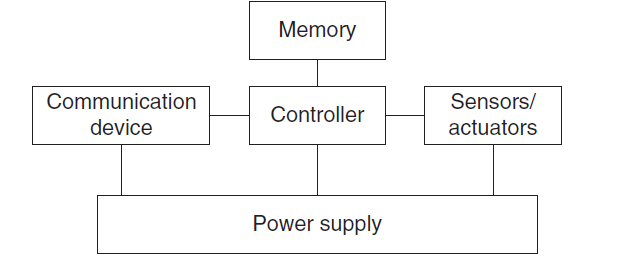
\includegraphics[width=10cm]{pictures/overview_node.png}
\caption{Visão Geral do Hardware de um Nó Sensor Sem Fio}
 \label{fig:overview}
\end{figure}

Nas próximas subseções serão apresentados, de forma resumida, alguns dos principais sensores existentes no mercado.

\subsubsection{Mica 2}
A plataforma \emph{Mica Mote} é comercializada pela \emph{Crossbow} e é uma das mais empregadas em projetos envolvendo RSSFs. A unidade de sensoriamento de cada nó \emph{Mica Mote} pode ser equipada com uma variedade de sensores, tais como acústico, temperatura, aceleração, luminosidade e pressão \cite{Ruiz2004}.

O \emph{Mica 2} é um nó sensor de baixo consumo de energia, podendo alcançar mais de um ano de autonomia utilizando pilhas AA. Este modelo possui um transceiver de rádio de 868/916 MHz multi-canal e utiliza \emph{Tiny OS} como sistema operacional.
O corpo deste sensor apresenta um conector de expansão de 51 pinos, isto permite que se conecte sensores de luz, temperatura, pressão, aceleração/sísmico, acústico, magnetismo, entre outros.

Devido suas características, o \emph{Mica 2} é indicado para aplicações como: segurança, vigilância, monitoramento de ambientes, redes de sensores de larga escala (mais de 1000 nós) e plataformas de computação distribuída.

Mais informações em: \cite{Mica2}.

\subsubsection{Mica Z}
O nó sensor \emph{Mica Z} é uma variação da plataforma \emph{Mica Mote}. Este nó possui diversas características comuns ao sensor \emph{Mica 2}, contudo, apresenta como suas maiores diferenças o uso de um rádio 2.4 GHz IEEE 802.15.4 e também sua capacidade de realizar transferências em taxas relativamente altas (250 kbps).

Este sensor pode ser utilizado em praticamente todos os tipos de aplicações do sensor \emph{Mica 2}. Em adição, este sensor é indicado para aplicações de medições acústica, de vídeo, vibração ou outras que demandem transmissões de alta taxa de transmissão, bem como aplicações de segurança e monitoramento \emph{indoor}.

Informações mais específicas podem ser encontradas em: \cite{MicaZ}.

\subsubsection{Iris}
Este modelo de nó sensor apresenta algumas características em comum com os nós da plataforma \emph{Mica Mote}, entretanto, apresenta avanços significativos em relação à plataforma anterior. Sua maior característica é o fato de possuir um rádio com alcance até três vezes maior que um sensor \emph{Mica Mote}, bem como o dobro de memória de programas.
Testes ao ar livre demonstraram que sensores utilizando esta plataforma foram capazes de se comunicar a uma distância de 500 metros.

Mais informações podem ser encontradas em: \cite{Iris}.

\subsubsection{TelosB}
\emph{TelosB} é uma plataforma \emph{Open Source} desenvolvida para permitir experimentação de ponta para a comunidade científica. Este sensor une diversas ferramentas essenciais para estudos de laboratório em um só sensor: Funcionalidade de programação via USB, um rádio IEE 802.15.4 com antena de integrada e uma CPU de baixo cosumo com memória extendida.
As características mais importantes deste nó sensor são a presença de interface USB para programação e uma memória flash externa de 1MB.

Informações mais detalhadas podem ser encontradas em: \cite{TelosB}.

\subsubsection{Imote 2}
O \emph{Imote 2} é uma plataforma avançada e de alto desempenho de nós sensores sem fio. Este modelo contém um processador Intel PXA271, com a capacidade de executar de baixas (16MHz) até frequências consideravelmente altas (416MHz).
Este tipo de sensor é indicado para aplicações que requeiram alto desempenho do nó sensor, como: processamento digital de imagens, monitoramento e análises industriais, monitoramento sísmico ou de vibração, etc.

Mais informações e características deste modelo podem ser visualizadas em: \cite{Imote}.


Na figura \ref{fig:nodes} podem ser visualizados os nós sensores citados nesta sessão.

\begin{figure}[h!]
\centering
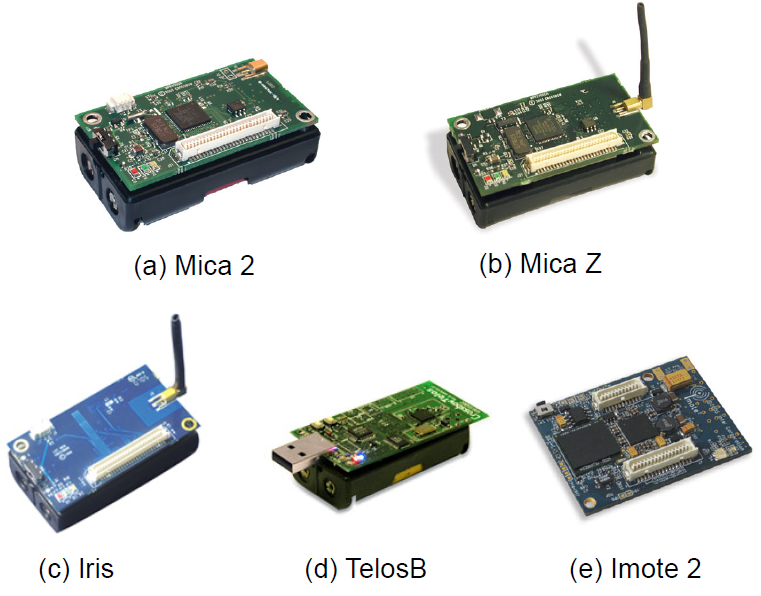
\includegraphics[width=12cm]{pictures/sensor_nodes.png}
\caption{Nós Sensores. (a) Mica 2, (b) Mica Z, (c) Iris, (d) TelosB, (e) Imote 2}
 \label{fig:nodes}
\end{figure}